\documentclass[12pt,a4paper]{report}
\usepackage{graphicx}
\usepackage{amsmath,amssymb}
\usepackage{geometry}
\usepackage{setspace}
\usepackage{fancyhdr}
\usepackage{pdfpages}
\usepackage{hyperref}
\usepackage{listings} % For code listings
\usepackage{listings-rust}
\usepackage{color}
\usepackage{url}
\usepackage{diagbox}

\geometry{margin=1in}
\setstretch{1.5}

% Custom commands
\newcommand{\HRule}{\rule{\linewidth}{0.5mm}}

% Title page
\title{
    \HRule \\[0.4cm]
    {\huge \bfseries  Efficient ZK Argument for Shuffle Implementation in Rust \\[0.4cm]}
    \HRule \\[1.5cm]
    \textsc{\Large Master's Thesis}\\[0.5cm]
    \textsc{\large University of Freiburg}\\[0.5cm]
}

\author{
    \Large Ahmet Ercem Bulut\\
    \Large Student ID: 5362638\\
    \Large Supervisor: Prof. Christian Schindelhauer
}

\date{August, 2024}

\begin{document}
% Decleration

\includepdf[pages={-}]{dec_signed.pdf}

% Title page
\maketitle
\thispagestyle{empty}
\newpage

% Abstract
\pagenumbering{roman}
\chapter*{Abstract}
\addcontentsline{toc}{chapter}{Abstract}
A shuffle operation in cryptography is an operation that takes a committed, anonymous series of values and returns the original serie modified with a permuted order. 
It is an important operation in many real world scenarios (e-voting, mental card games).
Due to the plaintexts or data being encrypted for privacy, the correctness of a shuffle of commitments is not straightforward to verify. While there are algorithms to construct such arguments, we are providing the first comprehensive 
pure Rust library for the Correctness of a Shuffle Operation.\par
The library is built over elliptic curve prime order groups 
to commit and encrypt data for privacy, while exploiting the homomorphism of the elliptic curves for efficiency.
This argument for correctness combines two separate arguments (Multi-exponentiation Argument, Product Argument) to produce a Shuffle Argument for correctness.\par 
Utilizing the Rust programming language, which has enormous support from the cryptography community, with its efficiency in runtime and security in memory, 
we aim to provide an extensive and easy to use zero-knowledge proof
framework that can be seamlessly incorporated and used by other proof schemes, or used to construct complex arguments.\par
We give performance results of the tests we ran as well to show the implementation follows the proposed optimized performance.\\
\textbf{Keywords:} rust, mix-net, zero-knowledge, shuffle, mental card games, elgamal

\newpage

% Acknowledgements
\chapter*{Acknowledgements}
\addcontentsline{toc}{chapter}{Acknowledgements}
I would like to start by thanking Prof. Christian Schindelhauer for his extensive guidance and infectious enthusiasm for cryptography.\par
Anneme ve Babama, koşulsuz destek ve sevgileri, ne kadar uzakta olsak da yalnız bırakmadıkları için,
Ablama, yıllar boyu bana örnek ve ideal olduğu için,
Dostlarıma, sayısız kahkahalar ve bana ögrettikleri için,\\
Sonsuza dek minnettarım.\par
A mis amigos, por llenar nuevas paginas con los recuerdos mas brillantes,\\
and to all the river nymphs, for help in the worst times and the melodies they sang,\par
Thank you.


\newpage

% Table of Contents
\tableofcontents

% List of Tables
%\newpage
%\listoftables

% Main content
\newpage
\pagenumbering{arabic}

\chapter{Introduction}
With the introduction of the Rust programming language to cryptography, there has been a sizable influx of cryptography research migrating to rust. 
The community has been at work creating tools and frameworks to exploit Rust's native advantages in performance and memory control. \par
We aim to contribute to this collection of tools and frameworks by implementing a secure and efficient version of a Shuffle Argument.
The Shuffle argument provided by Bayer and Groth \cite{bgshuffle} prove that a deck of "values" has been shuffled, with an honest zero-knowledge verifier that makes use of two independent arguments.\par
The sublinear communication complexity the argument provides is an improvement which is essential to smaller communications in proofs, and the main reason we want to combine this efficiency with the efficiency of the Rust Programming Language.\par
We will describe a library of arguments which ultimately combine into a complete and secure Bayer-Groth Shuffle Argument, 
and also be used in tandem with other cryptographic proofs and schemes provided by Rust's cryptograhic community.
\section{Bayer-Groth Shuffle Argument}
The Bayer-Groth shuffle argument \cite{bgshuffle}, is a specific type of zero-knowledge proof that
allows for the verification of correctness for a shuffle without revealing 
the underlying permutation or the original values. \par
This protocol is particularly useful in scenarios where data must be anonymized or shuffled 
securely, such as in electronic voting systems, secure auctions, and mental card games. \par
It enables a prover to demonstrate that a set of ciphertexts (encrypted values) is a valid 
permutation of another set of ciphertexts, with minimal computational and communication overhead.
The protocol achieves this by leveraging homomorphic encryption and prime order groups, ensuring that the shuffle's correctness can be verified without revealing any sensitive information or needing interaction.

\section{The Rust Programming Language}
Rust \cite{rust} is a near low-level programming language known for its emphasis on safety, concurrency and performance.
Designed to ensure properties that might be overlooked otherwise such as memory safety and
reference efficiency, Rust has quickly gained popularity in software development. 
Particularly for applications where performance and security are critical.\par
Rust's ownership model, which enforces strict rules on how memory is managed, ensures that programs
are both safe and efficient \cite{rust}. This is particularly important in cryptographic applications,
where errors in memory management can lead to vulnerabilities and exploits.\par
Rust's zero-cost abstractions and fine-grained control over system resources make it an ideal
choice for implementing complex cryptographic protocols, such as the Bayer-Groth shuffle argument.
\section{Previous Implementations and the Need for Rust}
While the Bayer-Groth shuffle argument has been implemented in various programming languages, 
there has been a growing interest in leveraging Rust’s unique features for cryptographic applications. \par
Existing implementations in languages like C++ or Python often face challenges related to memory safety, runtime performance or communication size.
Rust’s strict safety guarantees, combined with its ability to produce highly optimized binaries, make it an attractive choice for implementing cryptographic protocols.

\chapter{Related Work}
\section{Shuffle Arguments}
The shuffle operation has been introduced by Chaum \cite{cha81}, however a proof of correctness for the mix-nets has been troublesome to define over the years.
Argument defined by Desmedt and Kurosawa \cite{dk00} only accounted for a small scale corruption in the servers. Jakobson, Juels, and Rivest \cite{jjr02} proposed a relatively big number of servers to decrease the chance of leaks and tampered messages. 
Peng et al. \cite{pbdv04} limited possible permutations and required a ratio of senders to be honest. 
These drawbacks were addressed by Wikström \cite{wik02} and zero-knowledge arguments.\par
Zero-knowledge shuffles were flushed out by Sako and Killian \cite{sk95} and Abe \cite{abe98, abe99, ah01}. 
Furukawa and Sako \cite{fs01} and Neff \cite{nef01, nef03} created the first shuffle algorithms for ElGamal encrypted values with linear card count complexity.\par
Neff \cite{nef01} utilized the invraince of polynomials under permutation of roots to create the shuffle argument. Later Groth \cite{gro10} laid out a perfect honest verifier zero-knowledge protocol.
In 2008 Groth and Ishai \cite{gi08} proposed the first sublinear communication complexity shuffle argument. 
This was later improved on by Bayer and Groth \cite{bgshuffle} by decreasing the $\mathcal{O}(N^{\frac{2}{3}})$ communication complexity to $\mathcal{O}(N^{\frac{1}{2}})$, 
which was the most optimal solution until this year where Abdolmaleki et al. \cite{bpshuffle} managed to achieve logarithmic communication complexity with bulletproofs.\par

\section{Decaf: Eliminating cofactors through point compression}
Decaf \cite{decaf} proposes a point compression format for elliptic curves over 
large-characteristic fields. Which is an effective implementation of cofactor-4 elliptic curve points
used by many state of the art cryptographic libraries.\par
Prime order groups created by these elliptic curves show additive homomorphism. Which is a significant
improvement on performance when it comes to implementation of complex proofs.
\section{Existing Implementations}
\subsection*{Mental Poker}
Mental Poker \cite{mentalpoker} is a library aimed to implement a verifiable
mental poker game for research purposes. While it is also purely in Rust,
the library focuses more on the implementation and the efficiency of 
Barnett Smart Card Protocol \cite{Barnett}. They also differ in their choice
of cryptography primitives and go with arkworks curve points \cite{arkworks}. 
\subsection*{Bayer-Groth Mixnet}
A pure C++ implementation \cite{bgmixnet} of the protocol, for use in a messaging system.
Useful for us as well since they have in detail performance metrics we can
compare to. They use the same curve 25519 as ours and also give hardware specifications for the performances.\par
They have certain drawbacks such as: for some values of the parameter $m$ the 
verification fails, the row size $m$ should always be larger than the column size $n$ etc.. 
Our library works without these limitations as well.
\subsection*{groth-shuffle}
A simple implementation by Dalskov \cite{andshuf} in c++, using Rellic library for elliptic curve operations.
Kecchak algorithm for compressing the points, but no metrics or further elaborations are made.

\chapter{Objective and Structure}
Implementing the mathematical operations that construct a Shuffle argument is a trivial task with enough experience in programming. The main objective of this thesis is to utilize Rust's unique properties of memory safety and runtime efficiency to create a safe and verifiable library of arguments that is easy to use and incorporate.\par
By the end of the paper we hope to have given a convincing argument to why our library is secure and efficient, and also why Rust is a perfect match for such arguments of proof.
\section*{Thesis Structure}
In the remaining parts of the paper we will first talk about importand preliminary concepts. 
First we will talk about Pedersen commitment, ElGamal encryption, and their respective schemes.
We will also explain their homomorphism and how it could be exploited for arguments of knowledge.\par
We will go over Zero-Knowledge proofs and the schemes used in the shuffle argument.
Setting up for Bayer and Groth's shuffle argument, we will discuss how they achieved their optimized shuffle argument.
Finally we will describe Ristretto Points and how we incorporated it to our scheme.\par
In Implementation, we will explain our structure and try to show how we utilized, Rust's efficiency and safety for certain important parts of the protocol.\par
We will end our discussion with performance metrics we have collected and their significance,
followed by talking about what could be future additions to the library.
\chapter{Methodology}

\section{Pedersen Commitment}
Pedersen commitments are a cryptographic technique used to commit to a value 
while keeping it hidden, with the ability to later reveal the committed value. 
They are widely used in cryptographic protocols, including zero-knowledge proofs, 
due to their strong security properties and the ability to support homomorphic operations.
\subsection*{Key Components}
\begin{itemize}
	\item \textbf{Group Parameters:} Pedersen commitments rely on a cyclic group $G$ of prime order $q$, where the discrete logarithm problem is hard. Two generators $g$ and $h$ of the group are publicly known.
	\item \textbf{Commitment Value:} A value $C$ that commits to a message $m$ using a random blinding factor $r$.
\end{itemize}
\subsubsection{Commitment Process}
To commit a message $m$ (which is typically an integer modulo $q$), the commiter:
\begin{itemize}
	\item Chooses a random blinding factor $r$ uniformly from $\mathbb{Z}_q$.
	\item Computes the commitment $C$ as:\\ $C\,=\,g^m \cdot h^r \pmod q$
\end{itemize}
The commitment $C$ is then published, while $m$ and $r$ are kept secret.
\subsection*{Revealing the Commitment}
To reveal the commitment, committer discloses the values $m$ and $r$. 
The verifier checks the valididty by computing $C'\,=\,g^m \cdot h^r \pmod q$ and ensuring that $C'\,=\,C$.
\subsection*{Security}
\begin{itemize}
	\item \textbf{Hiding:} The commitment $C$ does not reveal any information about the message $m$ due to the random blinding factor $r$. This ensures privacy until the committer chooses to reveal the value.
	\item \textbf{Binding:} Once $C$ is published, the committer cannot change the value of $m$ without being detected, as doing so would require finding a different pair $(m,\,r)$ that produces the same commitment, which is infeasible due to the hardness of the discrete logarithm problem.
\end{itemize}
\section{ElGamal Encryption}
ElGamal encryption is a public-key cryptosystem based on the Diffie-Hellman key exchange \cite{elgamal}. The security of the encryption relies on the difficulty of solving the discrete logarithm problem in large cyclic groups. Without having the private key $x$, it is computationally infeasible to derive the plaintext from the ciphertext.
\subsection*{Key Components}
\begin{itemize}
	\item \textbf{Private Key:} A randomly chosen integer $x$, which is used to generate the public key. Needs to be secret.
	\item \textbf{Public Key:} Consists of a large prime number $p$, a genarator $g$ of a multiplicative group modulo $p$, and a public key $y$, where $y = g^x \pmod p$.
\end{itemize}
\subsubsection*{Encryption Process}
To encrypt a message $m$ (represented as a number), the sender:
\begin{itemize}
	\item Chooses a random integer $k$, which serves as the ephemeral key.
	\item Computes the ciphertext pair $(c_1, c_2)$ as follows:
		\begin{itemize}
			\item $c_1 = g^k \pmod p$
			\item $c_2 = m \cdot y^k \pmod p$
		\end{itemize}
\end{itemize}
The ciphertext $(c_1, c_2)$ is then sent to the recipient.
\subsubsection{Decryption Process}
The recipient, who knows the private key $x$, decrypts the ciphertext by:
\begin{itemize}
	\item Computing $s = c_{1}^{x} \pmod p$.
	\item Recovering the original message $m$ by computing $m = c_2 / s \pmod p$.
\end{itemize}
\subsubsection{Applications}
ElGamal encryption is used in various cryptographic protocols, including digital signatures and encryption schemes. 
Its ability to support homomorphic operations makes it particularly useful in privacy-preserving applications, 
such as secure voting systems and zero-knowledge proofs.
\section{Homomorphism}
Homomorphism refers to the ability of certain operations to respect the structure of the underlying group order. 
For example Pedersen commitments have additive homomorphism, which means any addition operation applied to the values before committing, would give the same result if the operation would have been applied to the commited versions of the same values.\par   
This characteristic is particularly valuable in scenarios where computations need to be performed on commited data without revealing it, preserving both privacy and security.\par
The Shuffle argument utilizes the homomorphism of both the Elgamal encryption and the Pedersen commitment.
\subsection*{Homomorphism of Pedersen Commitments}
Pedersen commitments' homomorphism as we mentioned is additive: the addition of two commitments is itself the commitment to the sum of the original messages.
Mathematically, if $C_1\,=\,g^{m_1}\,.\,h^{r_1}$ and $C_2\,=\,g^{m_2}\,.\,h^{r_2}$, then:\\ 
\begin{center}
$C_1\,+\,C_2\,=\,g^{m_1 + m_2} \cdot h ^{r_1 + r_2}$
\end{center}
This allows for multiple commited values to be combined in a way that reflects their arithmetic sum without revealing the individual values themselves.
\subsection*{Homomorphims of ElGamal Ciphertexts}
The shuffle argument involves showing that a set of ciphertexts (encrypted values) is a valid permutation of another set without revealing the permutation or the underlying plaintexts.\par
The usual definition of ElGamal encryption is over a finite field, where the homomorphism is multiplicative.
Homomorphims helps us achieve this via providing committed values that we can operate over rather than needing to reveal them in any way. Mathmetically:\\
The ciphertext $(c_1,\,c_2)$ of plaintext $m_1 \cdot m_2$:\\
\begin{center}
$(c_1, c_2) = \left( g^{k_1 \cdot k_2} \pmod p, \ (m_1 \cdot m_2) \cdot y^{k_1 \cdot k_2} \pmod p \right)$
\end{center}
with $k_1$ and $k_2$ being the respective ephemeral keys.\par
However, we are defining our ElGamal encryption over elliptic curves which turns their homomorphism towards addition like Pedersen commitments. This allows as tu treat encryption and commmitment primitives similarly and make sure they are in the same prime order.\par
Most of the proof construction algorithms' verification, efficiency and security is assured by using these properties for our arguments.

\section{Zero-Knowledge Proofs}
Zero-knowledge proofs (ZKPs) are a fundamental concept in cryptography, enabling one party 
(the prover) to demonstrate knowledge of a particular piece of information to another party 
(the verifier) without revealing the information itself.\par
This concept, first introduced by Goldwasser, Micali, and Rackoff \cite{zk}, has since become 
an important part of privacy-preserving cryptographic protocols. 
ZKPs are widely used in applications where privacy and security are paramount, 
such as digital signatures, identity verification, and secure voting systems.
\subsection*{Special honest verifier zero-knowledge argument of knowledge}
The zero-knowledge scheme that we are going to be using for our arguments(defined by Bayer and Groth) is defined over a common reference string $\sigma$ that is the result of a probabilistic polynomial time setup algorithm $\mathcal{G}$ dependent on a arbitrary security parameter.
Our common reference string is a tuple $\sigma = (pk, ck)$ where $pk$ and $ck$ are public key for the ElGamal encryption and commitment key for the Pedersen commitment.\par
The languages of statements $x$ are defined as the set of statements that have a witness $w$ for the relation $R$ under the common reference key. Meaning the shuffle is valid in the case of a shuffle argument, where $x$ is the original and shuffled deck, $w$ is the proposed permutation and the base hiding factor of the base ElGamal encryption.
\begin{center}
	$L_\sigma := \{x | \exists w : (\sigma, x, w) \in R\}$
\end{center}
The commitments revealed by communication create a public transcript, which is the result of algorithms such as the prover $\mathcal{P}$ and verifier $\mathcal{V}$ interacting with inputs. We will denote the transcript entries as $(\sigma, hist) \leftarrow \mathcal{G}(\lambda)$, where $\lambda$ is the security parameter for example.
One can think of the transcript as values needed for verification while remembering it is public and should not share open values. 
The last entry in this public transcript is the acceptance or rejection of the prover verifier duo.\par
An $argument$ is defined as a triple of the setup algorithm, prover and verifier: $(\mathcal{G}, \mathcal{P}, \mathcal{V})$.
This $argument$ when faced with an adversary $(x, w) \leftarrow \mathcal{A}(\sigma, hist)$, either accepts the argument via $\mathcal{P}(\sigma, x, w), \mathcal{V}(\sigma, x)$ accepting, 
or claims the statement and witness provided by the adversary is not in the relation $R$ and rejects. 
This implies perfect completeness.\par
The chance of an adversary fooling the verifier with an $x \notin L_\sigma$ and no witness, is computationally hard due to keeping a history of transcript and the common reference key for the language. It would need to solve the discrete log problem for elliptic curves.\par
An argument is called a public coin if the prover's messages need to adhere to random and independent messages of the verifier. These are called $challenges$ made by the verifier.
A public coin's randomness provides honesty to the prover's actions, otherwise random challenges made by the verifier couldn't be verified in the final transcript.

\subsection*{The Fiat-Shamir heuristic}
Fiat-Shamir heuristic proposed in 1987 \cite{fiat} aims to turn an interactive argument, prover and verifier communicate as two entities to create a healthy argument, into a non-interactive one. This means the prover wouldn't have to wait for externally communicated challenges during the construction of the proof.\par
Not being dependent on verifier for the construction of the proof also means the same proof could be verified by all verifiers, otherwise interactions with every seperate verifier which is a lot more complexity.\par
Non-interactivity is achieved by a secure random oracle creating challenges instead of the verifier. 
If the oracle returns a uniformly random answer to brand-new inputs this satisfies the randomness and independence property normally enforced by the verifier.
To achieve this the prover requests random challenges from the oracle and sends this challenge to individual verifiers with the proof.

\section{Efficient ZK Argument for Correctness of a Shuffle}
In 2012, Bayer and Groth \cite{bgshuffle} presented an algorithm with sublinear 
communication complexity for shuffling a deck of homomorphically encrypted values.
According to their findings, operations for an efficient sublinear size argument
show linearity in group elements when they are "in the exponent". \par
Using this adaptation, they constructed an efficient multi-exponentiation argument that shows a ciphertext
$C$ is the product of a set of known ciphertexts $C_1,...,C_N$ raised to a set of
hidden committed values. \par 
By reducing this bottleneck sublinearly, the argument 
gains significant improvement in performance ($\mathcal{O}(\sqrt{N})$).
They also provide other optimization and minor improvements over the prover computations.\par
The algorithms used in the Bayer-Groth paper construct the backbone of our library,
with optimizations that are products of using native Rust and its efficiency.\par
While describing the algorithms we will follow the multiplicative homomorphism as to keep notation consistent with Bayer-Groth's paper, 
however in the implementation multiplication and exponentiation turns into addition and multiplication.
Specifically the algorithm consists of 6 proof schemes, some used as components for others.
We will describe these arguments in terms of special honest zero-knowledge arguments we described previously for brevity, 
since the mathematical justifications of the algorithms are beyond the scope of this paper.\par
We will denote the prime order group used by commitment as $\mathbb{G}$ and write $\mathbb{H} = \mathbb{G} \times \mathbb{G}$ for ciphertexts.
$c_a = com_{ck}(a; r)$ indicates a commitment for the value $a$ with a random value of $r$.
$\mathcal{E}(a; b)$ represents the ElGamal encryption of the message $a$ with randomness $b$.
$x, y, z$ will be reserved for challenges of the Fiat-Shamir heuristic from now on.
Finally we show a permutation $\pi$ of $\vec{C}$ as $\vec{C}_\pi$.
\subsection*{Shuffle Argument} 
The main argument for proof of shuffle.
\begin{itemize}
	\item \textbf{Common Reference:} $pk, ck$.
	\item \textbf{Statement:} $\vec{C}, \vec{C'} \in \mathbb{H}^N$ with $N = mn$.
	\item \textbf{Witness:} $\pi \in \Sigma_N$ and $\vec{\rho} \in \mathbb{Z}^{N}_q$ so that $\vec{C'} = \mathcal{E}(\vec{1}; \vec{\rho})\vec{C}_\pi$
\end{itemize}
Where $N$ is the total card count.\par
The argument aims to exploit the sum of all ciphertexts being unchanged by a shuffle operation.
After three layers of homomorphic challenges to $\pi$, the results and the openings are used in a Product Argument, 
which would only hold if $\pi$ would be a correct shuffle.\par
These challenges are also used to prove that a challenged sum of $\vec{C}^{\vec{x}}$ would
equal to a sum of the permuted chipertexts with challenged $\pi$ exponents and challenged $\rho$ randomness.
This is the main improvement of Bayer-Groth argument and is the Multi-Exponentation Argument
\subsection*{Multi-Exponentiation Argument} An argument that shows correctness of prime-order group exponentiations. 
The argument gets rid of overhead matrix elements that are not needed for the argument by only focusing on the main diagonal product(as that mimics the permutation as it contains every ciphertext), instead of all of the diagonals. 
\begin{itemize}
	\item \textbf{Common Reference:} $pk, ck$.
	\item \textbf{Statement:} $\vec{C}_1,\ldots,\vec{C}_m \in \mathbb{H}^n$ and $C \in \mathbb{H}$ and $c_{A_1},\ldots,c_{A_m} \in \mathbb{G}$ where $m = \mu m'$.
	\item \textbf{Witness:} $A \in \mathbb{Z}_{q}^{n \times m}, \vec{r} \in \mathbb{Z}_{q}^{m}$ and $\rho \in \mathbb{Z}_q$ such that
		\begin{center}
			$\displaystyle C = \mathcal{E}_pk(1; \rho) \prod_{i=1}^m \vec{C}_{i}^{\vec{a_i}}$ and $\vec{c}_A = com_{ck}(A; \vec{r})$.
		\end{center}
\end{itemize}
With $\mu$ being the optimization factor.
\subsection*{Product Argument} An argument proving that the product of certain commited vector values have a particular product.
\begin{itemize}
	\item \textbf{Common Reference:} $pk, ck$.
	\item \textbf{Statement:} $\vec{c}_A \in \mathbb{G}^m$ and $b \in \mathbb{Z}_q$.
	\item \textbf{Witness:} $A \in \mathbb{Z}^{n \times m}, \vec{r} \in \mathbb{Z}_{q}^m$ such that
		\begin{center}
			$\vec{c}_A = com_{ck}(A; \vec{r})$ and $\displaystyle \prod_{i=1}^n \prod_{j=1}^m a_{ij} = b$
		\end{center}
\end{itemize}
Product argument engages in a Hadamard Product argument for column-wise commitments to the witness matrix and a Single Value Product argument for the element-wise commitments.
\subsection*{Hadamard Product Argument} An Hadamard product between two vectors of same dimensions is a vector which the elements of are element-wise products of the argument vectors.\par
The argument shows that, vectors of commited values have a particular result vector for their element-wise(hadamard) product.
\begin{itemize}
	\item \textbf{Common Reference:} $pk, ck$.
	\item \textbf{Statement:} $\vec{c_A}, c_b$.
	\item \textbf{Witness:} $\vec{a}_1,\ldots,\vec{a}_m,\vec{r}$, and $\vec{b}, s$ such that
		\begin{center}
			$\displaystyle \vec{c}_A = com_{ck}(A;\vec{r})\qquad c_b = com_{ck}(\vec{b}; s)\qquad \vec{b} = \prod_{i=1}^m \vec{a}_i$.
		\end{center}

\end{itemize}
Finally engages in a Zero Argument to assert equality between the products of challenged commitments and the challenged product $b$.
\subsection*{Zero Argument} For two set of commited vectors and a bilinear mapping of two vectors to scalar, Zero argument shows the resulting operation equals $0$. 
Important for showing equality via difference.
\begin{itemize}
	\item \textbf{Common Reference:} $pk, ck$.
	\item \textbf{Statement:} $\vec{c}_A, \vec{c}_B$ and a bilinear map $*: \mathbb{Z}_q^n \times \mathbb{Z}_q^n \rightarrow \mathbb{Z}_q$.
	\item \textbf{Witness:} $A = \{\vec{a}_i\}_{i=1}^m \in \mathbb{Z}^{n \times m}_q, \vec{r} \in \mathbb{Z}_q^m$, and $B = \{\vec{b}_i\}_{i=0}^{m-1}, \vec{s} = (s_0,\ldots,s_{m-1}) \in \mathbb{Z}_q^m$ such that
		\begin{center}
			$\displaystyle \vec{c}_A = com_{ck}(A; \vec{r}) \qquad c_b = com_{ck}(\vec{B}; \vec{s}) \qquad 0 = \sum_{i=1}^m \vec{a}_i * \vec{b}_{i-1}$.
		\end{center}
\end{itemize}
The $*$ mapping incorporates one of the 3 challenges to project the column vector values of $A$ and $B$ into a singular value and the argument only accepts when this value equals zero.
\subsection*{Single Value Product Argument} a 3-move argument of knowledge \cite{gro10}, which shows that a vector of committed values have a particular single product.
\begin{itemize}
	\item \textbf{Common Reference:} $pk, ck$.
	\item \textbf{Statement:} $c_a \in \mathbb{G}$ and $b \in \mathbb{Z}_q$.
	\item \textbf{Witness:} $\vec{a} \in \mathbb{Z}_q^n, r \in \mathbb{Z}_q$ such that
		\begin{center}
			$c_a = com_{ck}(\vec{a};r) \qquad$ and $\displaystyle \qquad b = \prod_{i=1}^n a_i$.
		\end{center}
\end{itemize}

\section{Ristretto Points}
A Ristretto Point is a cryptographic construction designed to create a
prime-order group from elliptic curves using Decaf \cite{decaf} on Edwards Curves, 
enhancing the security and efficiency of cryptographic operations. 
In the context of mental card games, Ristretto Points 
enable players to prove knowledge or 
possession of certain cards without revealing the cards themselves.

\subsection*{Prime-Order Group Properties}
Ristretto Points provide a prime-order group that simplifies 
mathematical operations and ensures predictable, 
secure behavior in cryptographic protocols.
A prime-order group over elliptic curves eliminates issues related to cofactor multiplication, which can complicate the implementation of secure protocols.
In mental card games, this property ensures that each card, represented as a Ristretto Point, interacts securely and predictably within the proof system.

\subsection*{Unique Encoding and Decoding}
One of the key features of Ristretto Points is their ability to encode and decode points on an elliptic curve in a way that eliminates ambiguities.
Each encoded point uniquely corresponds to a single group element, which is critical for maintaining the integrity of the cryptographic proofs.
This property ensures that each card in the mental card game, when encoded as a Ristretto Point, has a unique representation, preventing issues such as duplication or misidentification.

\subsection*{Implementation of Choice}
We have chosen Dalek Cryptography's crypto tools framework curve25519-dalek \cite{dalek:curve}
as library of choice due to multiple reasons.
As the library supports the homomorphic properties of such group points, and since it is based on elliptic curves it shows additive homomorphism.\par
The library is also used prominently by the Rust Cryptography community in 
implementations of all kinds of cryptographic proofs and arguments.(bulletproofs, r1cs etc...). This gives us the advantage of being easily implementable into already existing Ristretto Point systems.


\chapter{Implementation}
\section{Commitments and Encryptions}
Since Ristretto points are defined in elliptic curve groups, it differs from the usual uses of ElGamal over a finite field where the homomorphism is multiplicative. 
In elliptic curve groups homomorphism becomes additive \cite{decaf}.\par
This means when we talk about multiplication of a scalar and a group point we are not talking about cofactor multiplication, 
we are talking about raising the group point to a scalar power. Because of the same reason we don't have addition between 
a scalar value and a group point, since group point addition is an automorphism.
By having both of our Pedersen commitments and ElGamal encrpytions over the same prime order group we can have seamless interaction between them. 
Here are some of the terms we will use according to Ristretto implementation before we go into design.
\subsection*{Primitives and Operations}
\begin{itemize}
	\item A Scalar is an open integer which is not commited or hidden in anyway, shown with a lower-case letter.
	\item A Point is any elliptic curve point (a Ristretto Point), achieved via commitment or encryption, shown with a upper-case letter. 
	\item A Ciphertext is a tuple of points over the ristretto elliptic curve, achieved by ElGamal encrpytion.
\end{itemize}
These primitives are provided to us via the Ristretto and elgamal-rust \cite{egrust} libraries.\par
As for the operations, we have implemented mathematically notated operations such as, 
vector multiplication, matrix exponentiation as generic traits over data types.
More complex operations such as commitment and encryption are abstracted to the Common Reference.
Here are the operations we have implemented over these primitives.
\subsubsection{Vectors}
\begin{itemize}
	\item $\vec{x}\vec{y} = (x_1y_1,\ldots,x_ny_n)$ and corresponding exponentiation
	\item $\vec{x}\cdot\vec{y} = \sum_{i=1}^n x_iy_i$
\end{itemize}
\subsubsection{Ciphertexts}
\begin{itemize}
	\item For $\vec{M} = (M_1,\ldots,M_n)$ and $\vec{\rho} = (\rho_1,\ldots,\rho_n)\\ \mathcal{E}_{pk}(\vec{M}; \vec{\rho}) = (\mathcal{E}_{pk}(M_1;\rho_1),\ldots,\mathcal{E}_{pk}(M_m;\rho_m))$
	\item For ciphertexts $C$, $\displaystyle \vec{C}^{\vec{a}} = (C_1,\ldots,C_n)^{a_1,\ldots,a_n)^T} = \prod_{i=1}^n C_i^{a_i}$.
	\item For matrix $A \in \mathbb{Z}^{n \times m}_q$ with column vectors $\vec{a}_1,\ldots\vec{a}_m\\ \vec{C}^A = (\vec{C}^{\vec{a}_1},\ldots,\vec{C}^{\vec{a}_m})$.
\end{itemize}
\subsubsection{Commitments}
Our Pedersen commitments have their commitment key $ck$ as $n+1$ random generators and their base prime order group. 
This allows us to commit to maximum $n$ sized vectors, we can also commit to less then $n$ elements by setting the rest of the entries to zero.
\begin{itemize}
	\item For matrix $A \in \mathbb{Z}^{n \times m}_q$ with column vectors $\vec{a}_1,\ldots\vec{a}_m\\ com_{ck}(A; \vec{r}) = (com_{ck}(\vec{a}_1;r_1),\ldots,com_{ck}(\vec{a}_m; r_m))$
	\item For vector $\vec{a} \in \mathbb{Z}_q^N$ and $\vec{r} \in \mathbb{Z}_q^m$ where $N = mn\\ com_{ck}(\vec{a};\vec{r})$ operation allows vectors of values to be treated as matrices if the parameter sizes dont match,an operation over column vectors.
\end{itemize}
\section{System Design}
\subsection*{Arguments}
We have decided to abstract each argument to:
\begin{itemize}
	\item a struct containing the initial public statements and witnesses,
	\item member prove function for the construction of the proof arguments,
	\item member verify function that verifies the initial statement with the given proof.
\end{itemize}
As such we have six "Provers" for each argument defined in Bayer-Groth, for the arguments injected into others the parent argument's constructed proof also contains the child argument's proof. 
This injection is paralleled in the verification step of the arguments, where the child prover is needed for the child verification so the overall verification becomes complete and secure.
\subsubsection{The Random Oracle}
For our non-interactive random oracle we chose a cryptographically safe RNG based on the ChaCha stream cipher \cite{cha}. 
Which is an improved variant of Salsa20 \cite{salsa} cipher family. 
The Pseudo-RNG based on this cipher uses the underlying cipher generators to expand a key into a stream of pseudo random bytes.\par
Which satisfies our definition of a random oracle for the Fiat-Shamir heuristic. During the construction of the proofs, the challenges $x, y, z$ are requested as random scalars from this random oracle.
\subsection*{Public Transcript}
The public transcript consists of the committed or encrypted values that are shared publicly by the prover. 
It is used to make sure the prover is honest and also by the verifier to finally decide on the argument.\par
We abstracted the transcript to the Proof structs we have defined returning from the proof functions of our provers. This allows for not yet proven Provers to still be able to verify proofs constructed by other provers of the same kind.
\subsection*{Common Reference}
First we take a look at the common reference string key needed for commitments and encryptions. 
The construction of this key is in polynomial time respect to card count since we need $n+1$ random generator points from our group order $q$ for Pedersen commitments. 
The ElGamal public key is much less of a problem since its public key setup can be done in constant time.
To keep consistency with our group order for our commitments and encryptions we made sure to use the same Ristretto curve.\par
We also decided to abstract the common reference keys in a seperate struct. 
This component's associated
member functions also shouldered the responsibility for: 
\begin{itemize}
	\item returning random scalars from a crpytographically safe rng, 
	\item commiting scalars, vectors and matrices of scalars, 
	\item encryption of scalar or point values.
\end{itemize}
\subsection*{Provers}
So far we have our statement and witnesses as constructor arguments for our Provers, public transcript as the Proof structs created by prove methods, our verifier as a method verifying the proof structs and our common reference key as a seperate struct. We can see the implementation is complete with respect to special honest zero-knowledge argument of knowledge.\par
The operations made during prove are  mathmetical implementations of the Bayer-Groth algorithms. 
Rust provides us with security by keeping the statements, witnesses and the transcript explicitly immutable by keeping their fields private, 
fast batch operations are thanks to its efficient iterator and collection access implementations with zero-cost abstractions.
This property is especially exploited when it comes to matrix operations.\par
As shown in table \ref{table:diagon} the diagonalization over a factor of the total number of elements
can look pretty straight forward once the index arithmetics are manipulated for efficiency.
Since the matrix exponentiation here is purely defined via iterators in $pow()$, 
the iterative recalling of this function is devoid of indexed memory access overhead.\par
This type of improvements provided by native Rust is repeated in many places across the library.
All of the codebase is open on github \cite{repo}, accompanied with a comprehensive rust documentation.

\begin{table}
\begin{lstlisting}[language=Rust]
let m = //factor of card count(effective column count)
let mu = //Efficiency hyperparameter
let m_ = m / mu;//(Square root of N for optimal)
//Base Ciphertexts for diagonal products
//b_ and tau_ are random value scalar vectors
let mut randomCT: Vec<Ciphertext> = b_.iter()
	.zip(tau_.iter())
	.map(|(_b, _tau)| {
	    self.com_ref.encrypt(&EGInp::Scal(*_b) 
				  ,_tau)
	}).collect();

//Diagonal Operations over mu
for i in 1..=mu {
    for j in 1..=mu {
	let k = j + mu - i - 1 ;
	randomCT[k] = (0..=m_ - 1).fold(randomCT[k],
		    |acc, l|
			acc + self.C_mat[mu * l + i - 1].pow(self.A[mu * l + j - 1])
		   );
            }
        }
\end{lstlisting}
\caption{Diagonalization over $n\,X\,m$ matrix}
\label{table:diagon}
\end{table}

\section{Main Challenges}
The proof constructions become straight forward whence the common references are set. 
Since they are non-interactive as well the verifier part can be simulated by random challenges.
However due to multiple proof compositions, an $y$ challenge we have recieved in the parent proof,
should also be the same challenge in the child proof. We have decided that the challenges should be passed down in the proving step since composite proofs are still sequential.\par
Other than small design decisions as such, most of the effort went into designing the system according to zero-knowledge schemes and making sure of the soundness of the algorithms.
\chapter{Results}
We have measured the time it takes for any of the arguments' proof and verification, while also recording the resulting proofs' memory size. 
Even at first with low card count of $8 x 8\,=\,64$ in \ref{table:allresults} we can see how the optimized version of multi-exponentiation is much more efficient in both size and time performance.\par
Since the main improvement is the difference between this optimized and base versions we will focus on more test results with different parameters in \ref{table:mexp}.\par
As we can see from the table the proof size is dependent on the column size($m$) of a matrix of cards, rather than $N$ the total card count.
This is due to the efficiency of the shuffle argument, performing expensive operations over column vectors instead over single values.\par
While the speed of the base argument still is affected by the total card count, we can see that is not true for the optimized argument. The optimized argument is not even dependent on the column size but only on the efficency parameter $mu$.
We can see the performance metrics follow the proposed speed up and proof size in Bayer-Groth. A $\mathcal{O}(\sqrt{N})$\cite{bgshuffle} space improvement when $mu\,=\,1$.\par
\begin{table}
	\begin{center}
	\begin{tabular}{||c|c||}
		\hline
		Setup Time&41\\
		Permutation Time&40\\
		\hline
		m&8\\
		n&8\\
		mu&1\\
		\hline \hline
		Proof Type&Time(ms) or Size(bytes)\\
		\hline
		Shuffle Proof Size&10304\\
		Shuffle Proof Time&702\\
		Shuffle Verify Time&93\\
		\hline
		Opt Mexp Proof Size&1184\\
		Opt Mexp Proof Time&102\\
		Opt Mexp Verify Time&17\\

		Base Mexp Proof Size&8224\\
		Base Mexp Proof Time&551\\
		Base Mexp Verify Time&88\\
		\hline
		Product Proof Size&1648\\
		Product Proof Time&327\\
		Product Verify Time&75\\
		\hline
		SV Product Proof Size&1088\\
		SV Product Proof Time&31\\
		SV Product Verify Time&18\\
		\hline
		Hadamard Proof Size&5280\\
		Hadamard Proof Time&283\\
		Hadamard Verify Time&57\\
		\hline
		Zero Proof Size&3680\\
		Zero Proof Time&205\\
		Zero Verify Time&47\\
		\hline 
	\end{tabular}
	\end{center}
	\caption{Performance Metrics, Time in ms, Size as bytes}
	\label{table:allresults}
\end{table}

\begin{table}
	\begin{center}
	\begin{tabular}{||c|c|c||}\hline
		\backslashbox{Parameters}{Proof Type} & Base Mexp& Optimized Mexp\\
		\hline
		N=64; m=8; $mu$=1 & 8224/639 & 1184/119\\
		\hline
		N=64; m=8; $mu$=4 & 8224/631 & 4064/322 \\
		\hline
		N=128; m=8; $mu$=1 & 8480/1220 & 1184/211\\
		\hline
		N=128; m=16; $mu$=1 & 15904/2298 & 1184/221\\
		\hline
		N=128; m=16; $mu$=4 & 15904/2198 & 4064/600\\
		\hline
		N=1024; m=16; $mu$=1 & 17696/17544 & 1184/1779\\
		\hline
	\end{tabular}
	\end{center}
	\caption{Multi-Exponentiation Trials, Space(bytes)/Time(ms) metrics}
	\label{table:mexp}
\end{table}

We have also recorded a series of trials with different parameters of card count.
Every trial uses a different seed and random values for the cards with the only restriction being the cards need to fit into 128 bits.
We have only recorded square number of cards since that is the optimal environment for the algorithm, however the library can work with any non-prime number of cards.
We can see the overall space\ref{fig:space}, and time metrics of the trials\ref{fig:time}, follow the proposed improvements.

\begin{figure}[h]
	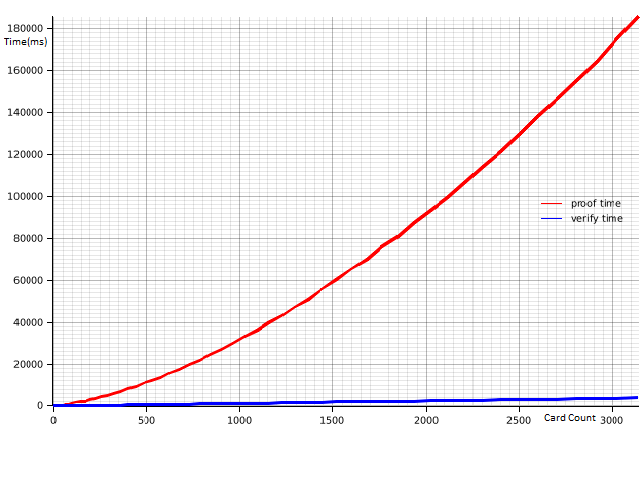
\includegraphics[scale=0.8]{time}
	\caption{Time(ms) Metrics}
	\label{fig:time}
\end{figure}

\begin{figure}[h]
	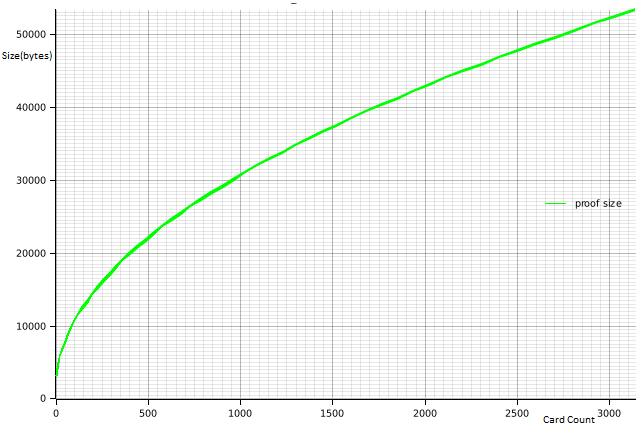
\includegraphics[scale=0.8]{space}
	\caption{Space(bytes) Metrics}
	\label{fig:space}
\end{figure}
\section{Implications}
We have achieved a safe and verifiable Rust library that constructs shuffle proofs.
Since we have used a common scheme for security, Ristretto Points, our arguments and proof construction algorithms could be implemented seamlessly to any Rust proof scheme.
Theoretically inspired by Bayer-Groth and practically useful with Rust we provide this easy to use shuffle argument library.\par
Providing modular implementations of every sub proof, that can be used to create more complex or simpler proofs than shuffling.
We are hoping this would provide the cryptography community in Rust with some inspiration.
\section{Limitations}
Bayer-Groth algorithm assumes pairs of ciphertexts are valid, while in practice there could be malicious adversaries switching ciphertexts pairs. the validity of the shuffled deck's ciphertexts should be checked externally.
While the Bayer-Groth algorithm suggests it works with any homomorphic property,
in our case we have only covered ElGamal encryption and Pedersen commitments over elliptic curves.\par
Some of the arguments don't have mutual dependencies so the overall Shuffle Argument performance
could be better if concurrency were added. However for a proof of concept we have not decided to implement it.
\chapter{Conclusion}
In conclusion we believe we have provided the first Rust library that implements a complete Zero-Knowledge Shuffle Argument, ensuring of the frameworks safety and soundness through zero-knowledge proof schemes and cryptographic primitives provided by Rust.
Because Rust's community is growing everyday there is an increasing demand in practical implementations of all kind, which we believe we have contributed to the cryptography discourse with this library.

\chapter{Future Work}
The library will be improved going forward with certain improvements already underway such as:
\begin{itemize}
	\item Generalized prove-verify schemes with Rust Traits
	\item Concurrency between Product Argument and Mexp Argument for a faster Shuffle Argument
	\item Generalized homomorphism, so any explicitly defined homomorphism is supported
\end{itemize}
There is also space for addition of mental card game utilities of creating decks, rounds and dealing.

% References
\newpage
\addcontentsline{toc}{chapter}{References}
\bibliographystyle{IEEEtran}
\bibliography{thesis}

% Appendix
\appendix
\chapter{Appendix A}
\section{ElGamal Encryption}

\subsection{Overview of ElGamal Encryption}
ElGamal encryption is a public-key cryptosystem based on the Diffie-Hellman key exchange. It ensures confidentiality and security under the assumption that the discrete logarithm problem is hard.

\subsection{Key Generation}
\begin{itemize}
    \item \textbf{Select Parameters:} A large prime \( p \) and a generator \( g \) of the multiplicative group \( \mathbb{Z}_p^* \).
    \item \textbf{Private Key:} A random integer \( x \) such that \( 1 \leq x < p-1 \).
    \item \textbf{Public Key:} Calculate \( y = g^x \pmod p \).
\end{itemize}
The public key is \( (p, g, y) \), and the private key is \( x \).

\subsection{Encryption Process}
To encrypt a message \( m \) (where \( m < p \)):
\begin{enumerate}
    \item Choose a random ephemeral key \( k \) such that \( 1 \leq k < p-1 \).
    \item Compute \( c_1 = g^k \pmod p \).
    \item Compute \( c_2 = m \cdot y^k \pmod p \).
\end{enumerate}
The ciphertext is \( (c_1, c_2) \).

\subsection{Decryption Process}
To decrypt the ciphertext \( (c_1, c_2) \) using the private key \( x \):
\begin{enumerate}
    \item Compute \( s = c_1^x \pmod p \).
    \item Compute \( m = c_2 \cdot s^{-1} \pmod p \), where \( s^{-1} \) is the multiplicative inverse of \( s \) modulo \( p \).
\end{enumerate}
The result \( m \) is the original plaintext message.

\subsection{Homomorphic Properties}
ElGamal encryption has a multiplicative homomorphism property. Given two ciphertexts \( (c_{11}, c_{12}) \) for message \( m_1 \) and \( (c_{21}, c_{22}) \) for message \( m_2 \), the product of these ciphertexts is a valid encryption of the product \( m_1 \cdot m_2 \):
\[
(c_{11} \cdot c_{21} \pmod p, \ c_{12} \cdot c_{22} \pmod p) = \left( g^{k_1 + k_2} \pmod p, \ (m_1 \cdot m_2) \cdot y^{k_1 + k_2} \pmod p \right)
\]

\section{Pedersen Commitments}

\subsection{Overview of Pedersen Commitments}
Pedersen commitments are a cryptographic primitive that provides a way to commit to a value while keeping it hidden and allowing the commitment to be opened later. They are homomorphic, additively hiding, and computationally binding, making them useful in various cryptographic protocols.

\subsection{Commitment Scheme}
Given a cyclic group \( G \) of prime order \( q \) with a generator \( g \) and another element \( h \) where the discrete logarithm of \( h \) with respect to \( g \) is unknown:
\begin{itemize}
    \item \textbf{Commitment:} To commit to a value \( m \), choose a random \( r \in \mathbb{Z}_q \) and compute the commitment as:
    \[
    C = g^m \cdot h^r \pmod q
    \]
    Here, \( C \) is the commitment, \( m \) is the message, and \( r \) is the random blinding factor.
\end{itemize}

\subsection{Opening the Commitment}
To open the commitment \( C \), reveal both the value \( m \) and the blinding factor \( r \). The verifier can check the validity of the commitment by recomputing \( C \) as:
\[
C' = g^m \cdot h^r \pmod q
\]
If \( C' = C \), the commitment is valid.

\subsection{Homomorphic Properties}
Pedersen commitments are homomorphic, meaning the product of two commitments is a commitment to the sum of the corresponding values. For two commitments \( C_1 = g^{m_1} \cdot h^{r_1} \) and \( C_2 = g^{m_2} \cdot h^{r_2} \), the combined commitment is:
\[
C_1 \cdot C_2 = g^{m_1 + m_2} \cdot h^{r_1 + r_2} \pmod q
\]
This property allows for operations on committed values without revealing them.

\subsection{Security Properties}
Pedersen commitments are:
\begin{itemize}
    \item \textbf{Hiding:} The commitment does not reveal the value \( m \) due to the random blinding factor \( r \).
    \item \textbf{Binding:} It is computationally infeasible to find different pairs \( (m, r) \) and \( (m', r') \) such that \( g^m \cdot h^r = g^{m'} \cdot h^{r'} \).
\end{itemize}
These properties make Pedersen commitments highly secure for use in zero-knowledge proofs and other cryptographic protocols.
\end{document}

